\chapter{System architecture}
\label{cha:architecture}


% --------------------------------------------------------------------------- %
% Files
% --------------------------------------------------------------------------- %
\section{Files}
\label{sec:files}

The files of our system can be divided into three parts:


\subsection*{Input files} % ------------------------------------------------- %

\begin{description}
\item[Legemiddelhåndboka HTML]
The HTML files of the Legemiddelhåndboka.

\item[ICD/ATC owl2 files]
The owl2 ontologies we use in our solution for classification.

\item[Patient cases text files]
Textfiles of the patient cases.
\end{description}


\subsection*{Java classes} % ------------------------------------------------ %

%\hyperref[fig:class-diagram]{Figur \ref*{fig:class-diagram}

\begin{description}
\item[Program]
This the main class that calls the parsers to retrieve information, it also does
the rankings.

\item[Chapter]
This class contains the information for a Legemiddelhåndbok chapter. Also
contains a list of subchapters.

\item[PatientCase] This class contains the information for a patient case.

\item[HandbookParser]
This class parses the information from the Legemiddelhåndboka HTML files and
creates chapter objects.

\item[OntologyClassificator]
This class has all the icd documents indexed, we can add new documents or we can
search among them with a query.

\item[OWL\_Class]
Contains the information of a class in an owl ontology.

\item[Owl\_Class\_Array]
Is an array of Java OWL classes.

\item[OwlParser]
Parses an ontology into an array of Java OWL classes.

\item[PatientCaseParser]
Read a patient case and return a new PatientCase object.
\end{description}

\begin{figure}[htb]
\begin{center}
    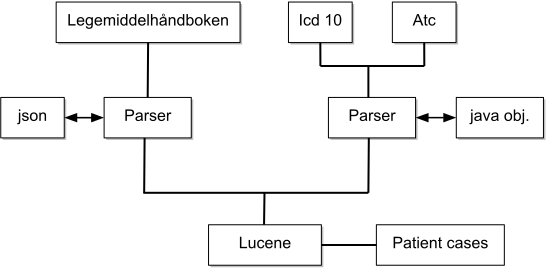
\includegraphics[width=\textwidth]{figures/class-diagram}
\end{center}
\caption{Class diagram}
\label{fig:class-diagram}
\end{figure}


\subsection*{Output files} % ------------------------------------------------ %

\begin{description}
\item[allchapters.json]
The Legemiddelhåndboka chapters in json format.

\item[atc.owl\_parsed \& ICD-10no.owl\_parsed]
The OWL ontologies as a serialized object.
\end{description}


% --------------------------------------------------------------------------- %
% Parts
% --------------------------------------------------------------------------- %
\section{Parts}
\label{sec:parts}

\hyperref[fig:system-overview]{Figure \ref*{fig:system-overview}} shows an
overview of the system components. The system can be split into five logical
parts:

\subsection*{Legemiddelhåndboka parsing}

Does all the parsing of Legemiddelhåndboka as well as creating java objects of
the chapters. Contains methods of retrieving these chapters.

\subsection*{Owl2 parsing}

Parses ontologies and save it in java objects.

\subsection*{Patient case parsing}

Reads the patient cases and save them in java objects.

\subsection*{Classification}

This part of the system is used for getting relevant ontology codes(icd or atc
codes). This part uses Lucene.

\subsection*{Ranking}

This part use the classification to get codes and use these codes to match
chapters and patient cases. This part uses Lucene.


\begin{figure}[htb]
\begin{center}
	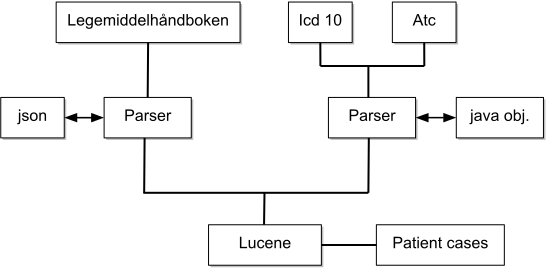
\includegraphics[width=\textwidth]{figures/system-overview}
\end{center}
\caption{System overview}
\label{fig:system-overview}
\end{figure}

% --------------------------------------------------------------------------- %
% External libraries
% --------------------------------------------------------------------------- %
\section{External libraries}
\label{sec:external-libraries}

\subsection*{Jsoup}
Jsoup is an open source Java library for working with real-world HTML. It
provides a very convenient API for extracting and manipulating data. We use
Jsoup during the parsing of Legemiddelhåndboka.\\\\
\url{http://jsoup.org/}

\subsection*{The OWL API}
The OWL API is an open source Java library used when working with OWL
ontologies. We use this API when we’re retrieving information from the ICD-10
OWL ontology.\\\\
\url{http://OWLAPI.sourceforge.net/}

\subsection*{JSON.simple}
JSON simple is a Java toolkit that are used to encode/decode JSON text. We use
this to when we want to save the chapters of Legemiddelhåndboka. We chose
JSON.simple because it provides a very simple and basic tool to convert Java
objects to JSON text, which is just what we needed.\\\\
\url{https://code.google.com/p/json-simple/}

\subsection*{Lucene}
Apache Lucene is an open source text search engine library written in Java. We
use Lucene for all our indexing/searching operation in our solution.\\\\
\url{http://Lucene.apache.org/core/}

% vim: set ts=2 sw=2 tw=80:
